%% Basierend auf einer TeXnicCenter-Vorlage von Tino Weinkauf.
%%%%%%%%%%%%%%%%%%%%%%%%%%%%%%%%%%%%%%%%%%%%%%%%%%%%%%%%%%%%%%

%%%%%%%%%%%%%%%%%%%%%%%%%%%%%%%%%%%%%%%%%%%%%%%%%%%%%%%%%%%%%
%% HEADER
%%%%%%%%%%%%%%%%%%%%%%%%%%%%%%%%%%%%%%%%%%%%%%%%%%%%%%%%%%%%%
\documentclass[ paper=a4,
    twoside=false,
    fontsize=12pt,
    pagesize=auto,
    parskip=half,
    % Linie unterhalb der Kopfzeile
    headsepline=true,
    % Kapitelnummern (in Kopfzeile), Bildunterschrift und Tabellen�berschriften erhalten keinen abschlie�enden Punkt. Alternative: enddot
    numbers=noenddot,
    % Markiert zu lange und zu kurze Zeilen. Die PDF-Datei enth�lt au�erdem keine klickbaren Links mehr.
    draft=false]{scrartcl}
% Alternative Optionen:
%	Papiergr��e: a4paper / a5paper / b5paper / letterpaper / legalpaper / executivepaper
% Duplex: oneside / twoside
% Grundlegende Fontgr��en: 10pt / 11pt / 12pt
\usepackage{setspace}
\usepackage[font=small,labelfont=bf,labelsep=endash,format=plain]{caption}
\usepackage[square,numbers]{natbib} %f�r Biblographierung
\bibliographystyle{unsrtnat}
\usepackage{array,dcolumn}
\usepackage[colorlinks,
pdfpagelabels,
pdfstartview = FitH,
bookmarksopen = true,
bookmarksnumbered = true,
linkcolor = black,
plainpages = false,
hypertexnames = false,
citecolor = black] {hyperref} % Verweiseim PDF
\usepackage{bookmark}
\usepackage{microtype} % optische verbesserung
\usepackage{booktabs} % Tabellen tool
\usepackage{float}	% For Bilder
\usepackage{subcaption} % Bilder nebeneinander

\usepackage{xcolor}
\usepackage{svg}
\usepackage{import}
%\usepackage[utf8]{inputenc}




%% Deutsche Anpassungen %%%%%%%%%%%%%%%%%%%%%%%%%%%%%%%%%%%%%
\usepackage[ngerman,english]{babel}
%\usepackage[latin1]{inputenc}
\usepackage[T1]{fontenc}% Silbentrennung bei Sonderzeichen

\usepackage[ansinew]{inputenc} % Direkte Angabe von Umlauten im Dokument.
\usepackage{lmodern} %Type1-Schriftart f�r nicht-englische Texte
\usepackage[babel, german=quotes]{csquotes} %,,''

%% Packages f�r Grafiken & Abbildungen %%%%%%%%%%%%%%%%%%%%%%
\usepackage{graphicx} %%Zum Laden von Grafiken
%\usepackage{subfig} %%Teilabbildungen in einer Abbildung
%\usepackage{pst-all} %%PSTricks - nicht verwendbar mit pdfLaTeX
\usepackage{units}

%% Beachten Sie:
%% Die Einbindung einer Grafik erfolgt mit \includegraphics{Dateiname}
%% bzw. �ber den Dialog im Einf�gen-Men�.
%% 
%% Im Modus "LaTeX => PDF" k�nnen Sie u.a. folgende Grafikformate verwenden:
%%   .jpg  .png  .pdf  .mps
%% 
%% In den Modi "LaTeX => DVI", "LaTeX => PS" und "LaTeX => PS => PDF"
%% k�nnen Sie u.a. folgende Grafikformate verwenden:
%%   .eps  .ps  .bmp  .pict  .pntg


%% Packages f�r Formeln %%%%%%%%%%%%%%%%%%%%%%%%%%%%%%%%%%%%%
\usepackage{amsmath}
\usepackage{amsthm}
\usepackage{amsfonts}


%% Zeilenabstand %%%%%%%%%%%%%%%%%%%%%%%%%%%%%%%%%%%%%%%%%%%%
%\usepackage{setspace}
%\singlespacing        %% 1-zeilig (Standard)
%\onehalfspacing       %% 1,5-zeilig
%\doublespacing        %% 2-zeilig


%% Andere Packages %%%%%%%%%%%%%%%%%%%%%%%%%%%%%%%%%%%%%%%%%%
%\usepackage{a4wide} %%Kleinere Seitenr�nder = mehr Text pro Zeile.
%\usepackage{fancyhdr} %%Fancy Kopf- und Fu�zeilen
%\usepackage{longtable} %%F�r Tabellen, die eine Seite �berschreiten
\usepackage{scrlayer-scrpage}

%%%%%%%%%%%%%%%%%%%%%%%%%%%%%%%%%%%%%%%%%%%%%%%%%%%%%%%%%%%%%
%% Anmerkungen
%%%%%%%%%%%%%%%%%%%%%%%%%%%%%%%%%%%%%%%%%%%%%%%%%%%%%%%%%%%%%
%
% Zu erledigen:
% 1. Passen Sie die Packages und deren Optionen an (siehe oben).
% 2. Wenn Sie wollen, erstellen Sie eine BibTeX-Datei
%    (z.B. 'literatur.bib').
% 3. Happy TeXing!
%
%%%%%%%%%%%%%%%%%%%%%%%%%%%%%%%%%%%%%%%%%%%%%%%%%%%%%%%%%%%%%


%%%%%%%%%%%%%%%%%%%%%%%%%%%%%%%%%%%%%%%%%%%%%%%%%%%%%%%%%%%%%
%% Optionen / Modifikationen
%%%%%%%%%%%%%%%%%%%%%%%%%%%%%%%%%%%%%%%%%%%%%%%%%%%%%%%%%%%%%

%\input{optionen} %Eine Datei 'optionen.tex' wird hierf�r ben�tigt.
%% ==> TeXnicCenter liefert m�gliche Optionendateien
%% ==> im Vorlagenarchiv mit (Datei | Neu von Vorlage...).
% Bisherige Einstellungen f�r Kopf- und Fu�zeilen l�schen:
\newcommand{\cImage}[2][0.5]{
	\begin{figure}[h!]
		\centering
		\includegraphics[width=#1\textwidth]{#2}
	\end{figure}
}
\RedeclareSectionCommand[style=section,indent=0pt,font=\usekomafont{partnumber}]{part}
\renewcommand*{\partformat}{\thepart\enskip}

  \newcaptionname{ngerman}\equationname{Formel}%
  \newcaptionname{ngerman}\listequationname{Formelverzeichnis}%

% Zentriert auf linken Seiten die aktuelle Kapitel�berschrift,
% auf rechten Seiten die �berschrift des aktuellen Abschnitts ausgeben:

% Zentriert die Seitenzahl ausgeben (auch beim Seitenstil "scrplain"):
\cfoot*{\pagemark}


%%%%%%%%%%%%%%%%%%%%%%%%%%%%%%%%%%%%%%%%%%%%%%%%%%%%%%%%%%%%%
%% DOKUMENT
%%%%%%%%%%%%%%%%%%%%%%%%%%%%%%%%%%%%%%%%%%%%%%%%%%%%%%%%%%%%%
\begin{document}
\selectlanguage{ngerman}
	\onehalfspacing
	\addtokomafont{sectioning}{\rmfamily}
	\numberwithin{equation}{section}
	\addtokomafont{caption}{\small\linespread{1}\selectfont}


\ihead{Theo Zwahlen}
\chead{}
\ohead{Rotorblattenteisung}

%% Deckblatt %%%%%%%%%%%%%%%%%%%%%%%%%%%%%%%%%%%%%%%%%%%%%%%%
%% ==> Schreiben Sie hier Ihren Text oder f�gen Sie eine externe Datei ein.

%% Die sch�nere Version:
\pagestyle{scrheadings} %%Keine Kopf-/Fusszeilen auf den ersten Seiten.
\begin{titlepage}

\begin{center}
\textbf{Industrieprojekt}\\
\vspace{15mm}

\textbf{\Huge Rotorblattenteisung}\\[2ex]
\textbf{Theo Zwahlen}\\
\vspace{40mm}


\begin{tabular}{ll}
Dozent:  & \quad Prof. Dr. Christoph Eck\\[1ex]
Experte: & \quad Prof. Dr. Th. Prud'homme\\[1ex]
Industriepartner: & \quad Aeroscout GmbH\\
 &\quad Hr. MSc Benedikt Imbach\\[1ex]
Abteilung: & \quad Elektrotechnik \& Informationstechnologie\\
 &	\quad Hochschule Luzern , Technik und Architektur\\
Abgabedatum: & \quad 21.\,Dezember\,2018\\
Geheimhaltungsstufe: & \quad R�cksprache
\end{tabular}

\end{center}

\end{titlepage}

%%\date{} %%Wenn kommentiert, wird das aktuelle Datum verwendet.
	%% , in Tabellen untereinander stellen
	%\newcolumntype{,}{D{,}{,}{-1}}
	%% +- in Tabellen untereinander stellen
	%\newcolumntype{p}{D{p}{\pm}{-1}}
%
%
	% %%Eine Datei 'deckblatt.tex' wird hierf�r ben�tigt.
%% ==> TeXnicCenter liefert eine m�gliche Deckblattdatei
%% ==> im Vorlagenarchiv mit (Datei | Neu von Vorlage...).
\newpage
\vspace*{90mm}
\large
\textbf{Selbstst�ndigkeitserkl�rung}\\


\emph{Hiermit erkl�re ich, dass ich die vorliegende Arbeit selbstst�ndig angefertigt habe und keine anderen als die angegebenen Hilfsmittel verwendet habe. S�mtliche verwendeten Textausschnitte, Zitate oder Inhalte anderer Verfasser wurden ausdr�cklich als solche gekennzeichnet.}\vspace{6mm}\\
\begin{tabular}{lp{8cm}r}
\small
Ort,& Datum & Unterschrift\\[4px]
\large
Horw,& 20. Dezember 2018& \\
\end{tabular}
\normalsize
\newpage


\addsec{Abstract}
%\addcontentsline{toc}{section}{Abstract}

\addsec{Kurzfassung}


\newpage

%% Inhaltsverzeichnis %%%%%%%%%%%%%%%%%%%%%%%%%%%%%%%%%%%%%%%
\tableofcontents %Inhaltsverzeichnis
\cleardoublepage %Das erste Kapitel soll auf einer ungeraden Seite beginnen.

\pagestyle{scrheadings} %%Ab hier die Kopf-/Fusszeilen: headings / fancy / ...



%% Kapitel / Hauptteil des Dokumentes %%%%%%%%%%%%%%%%%%%%%%%
%% ==> Schreiben Sie hier Ihren Text oder f�gen Sie externe Dateien ein.

%\input{intro} %%Eine Datei 'intro.tex' wird hierf�r ben�tigt.

%%%%%%%%%%%%%%%%%%%%%%%%%%%%%%%%%%%%%%%%%%%%%%%%%%%%%%%%%%%%%
%% ==> Im folgenden ein paar Hinweise:


\section{\textit{Vorwort}}
\textit{
Ich m�chte mich herzlich bei Prof. Dr. Christoph Eck f�r das Vertrauen und die Betreuung meiner Arbeit bedanken. Ausserdem danke ich Prof. Erich Styger f�r die Beratung und Hilfe im Bereich der Softwareerstellung. Ein grosses Dankesch�n geht an Robert Presel von der ETH Z�rich f�r die Unterst�tzung beim Gebrauch der Klimakammer. Weiter bedanke ich mich herzlich bei Romeo Bee f�r die Zusammenarbeit.}

\part{Einf�hrung}


\section{Einleitung}\label{Einleitung}

Aeroscout entwickelt Helikopter Drohnen f�r diverse Aufgaben\cite{Aeroweb}. Zuk�nftig sollen die Drohnen f�r Fl�ge im Hochgebirge eingesetzt werden. Dabei sind Anwendungen im Bereich der Bergrettung und der k�nstlichen Lawinenausl�sung im Fokus. Heute werden solche Fl�ge mit bemannten Hubschraubern oder gar nicht ausgef�hrt. Fl�ge mit bemannten Hubschraubern sind sehr teuer und bei nur kleinen Risiken wird auf Fl�ge verzichtet. Ein Drohnenflug ist im Vergleich billiger und wenn bei kritischen Wetterbedingungen Fl�ge m�glich w�ren, w�re das ein sehr grosser Vorteil.
Dazu m�ssen die Drohnen aber extremen meteorologischen Bedingungen standhalten k�nnen. Ein grosses Problem stellt dabei die Vereisung der Rotorbl�tter dar. Durch die Formver�nderung, die dadurch am Rotorblatt erfolgt, ist die Aerodynamik gest�rt und die Drohne wird innert K�rze flugunf�hig.
Diese Arbeit soll daher die Grundlage schaffen, um solche Vereisungen zu vermeiden. Sie erfolgt in enger Zusammenarbeit mit Romeo Bee von der Maschinentechnik. Seine Projektarbeit bezieht sich auf die Fertigung eines neuen Heckrotorblatts, in welches die n�tigen Enteisungsmassnahmen integriert sein sollen. Die vorliegende Arbeit bezieht sich vorwiegend auf die elektrischen Systeme zur Ansteuerung der Enteisung und die n�tige Infrastruktur f�r Versuchsaufbauten.

\section{Aufgabestellung}\label{Aufgabestellung}

F�r den Heckrotor soll der Prototyp einer Enteisungsvorrichtung entwickelt werden. Dies beinhaltet die Recherche �ber bestehende Systeme, die Ausarbeitung von m�glichen L�sungsans�tzen und die Realisierung eines Testaufbaus mit dem Heckrotor. Nach M�glichkeit soll die Funktion bei verschiedenen Temperaturen und bei verschiedenen Luftfeuchtigkeiten aufgezeigt werden.

\subsection{Problemaufspaltung} 
Die Aufgabenstellung kann in drei Teilprobleme unterteilt werden. Ein Teil ist die Enteisung als solches. Wie l�sst sich Eisbildung verhindern oder wie entfernt man bereits gebildetes Eis.
Eine weitere Teilaufgabe besteht in der Detektion der Problematik. Welche Messungen sind n�tig um Vereisung oder Vereisungsbedingungen sicher zu erkennen und darauf reagieren zu k�nnen.
Die letzte Teilaufgabe beinhaltet den Aufbau des Prototyps mit Bau und Anschaffung der n�tigen Elektronik und die Programmierung der n�tigen Software.

\section{Eisverhinderung}
Systeme zur Enteisung von Rotorbl�ttern lassen sich in zwei Arten unterteilen. Die eine heisst anti-icing. Dies sind Systeme, die das Rottorblatt durchgehend eisfrei halten. Das ben�tigt in vielen F�llen einen hohen Energieaufwand. Die Alternative heisst de-icing. Dabei bildet sich Eis �ber eine definierte Zeit. Anschliessend l�st das System das Eis vom Rotor und die Fliehkraft schleudert es weg. So kann ein erheblicher Teil der n�tigen Energie eingespart werden\cite{Pumapp}. Ein Nachteil dabei ist, dass das gebildete Eis bereits Einfl�sse auf das Flugverhalten haben kann. Dazu kommt die Gefahr von Besch�digung am Flugobjekt durch abgel�ste Eisst�cke.

\subsection{Oberfl�chenstruktur}
Ein Ansatz ist, den Rotor mit einer Oberfl�chenstruktur zu fertigen, welche kein Ansetzen von Eis zul�sst. Bis heute gibt es jedoch keine Oberfl�che, die diese Anforderung erf�llt. Die Vereisung l�sst sich durch Oberfl�chenstrukturen vermindern, jedoch nicht ganz ausschliessen. Weiter haben die Strukturen kurze Lebensdauern und sind schwer zu �berpr�fen.\cite{Frhofweb2}

\subsection{Mechanische Eisabl�sung}
Eine Methode, die bei kleineren Flugzeugen im Einsatz ist, l�st das Eis durch mechanische Verformung. Luftdruck bl�ht an der Fl�gelvorderkante angebrachte Luftkissen auf und sprengt so das Eis weg. Die Methode beinhaltet zwei wesentliche Schwierigkeiten. Zum einen m�sste die Verformung genau im richtigen Moment erfolgen. Es muss sich bereits Eis gebildet haben, dieses darf aber die Flugf�higkeit der Drohne nur minimal beeinflussen. Weiter sind die n�tigen Konstruktionen f�r eine solche Vorrichtung an einem drehenden Rotor sehr aufw�ndig.\cite{AeroGuideweb2}

\subsection{Elektrische Beheizung}
Die in der Aviatik etablierten Systeme basieren auf elektrischem Beheizen. So l�sst sich de- und anti-icing umsetzten. Beim Superpuma, ein Hubschrauber welche die Schweizer Armee einsetzt, sind die Rotoren mit Heizwiderst�nden ausger�stet. Der Hauptrotor ist mit einem elektrischen de-icing-System ausgestattet. Der Heckrotor verf�gt jedoch �ber ein elektrisches anti-icing System, um Sch�den durch gel�ste Eisst�cke am Hauptrotor oder am Rumpf des Hubschraubers zu vermeiden.\cite{Pumapp}
\newpage

\subsubsection{CNT-Farbe}
Carbon Nanotube (CNT) sind leitf�hige Fasern aus Kohlenstoff mit Durchmessern im Nanometerbereich. In Lacken und Kunststoffen gel�st f�hren sie zu elektrischer Leitf�higkeit. Die Fraunhofer-Gesellschaft bietet CNT Material in Form einer wasserbasierten Dispersion als Farbe oder Lack an. Die Farbe erzeugt eine homogene Erw�rmung auf der aufgetragenen Fl�che nach Anlegen von elektrischer Spannung\cite{Frhofweb}. �ber die Abriebfestigkeit der Dispersion gibt die Fraunhofer-Gesellschaft keine Auskunft. Eine Verarbeitung am Rotorblatt scheint ung�nstig. An der Oberfl�che aufgetragen sind die mechanischen Anspr�che zu hoch f�r einen langlebigen Betrieb. Eine Einarbeitung in Schichten des Rotorblatts ist schwierig zu realisieren.

\subsubsection{Textile Heizelemente}
Die Forster Rohner AG stellt textile Heizelemente her\cite{ForstRoweb}. Mit maximal 0.1\(\frac{W}{cm^2}\)\cite{ForstRoweb} ist die Leistung f�r eine Enteisung viel zu gering. Das Verfahren zur Einarbeitung von Heizelementen in Stoffe k�nnte jedoch gegebenenfalls auch zur Einarbeitung in die Karbonlagen des Rotorblattes als Grundlage dienen. Der technische Partner von Forster Rohner, die Firma Interactive Wear, gibt keine Auskunft �ber Herstellungsverfahren.

\subsection{Beheizen durch Abw�rme}
Eine M�glichkeit besteht darin, die Abw�rme des Hauptmotors direkt zum Beheizen des Rotors zu verwenden. Bei einigen Flugzeugen eingesetzte Methoden, bedienen sich genau dieses Konzepts. Dabei ist im Fl�gel des Flugzeuges eine Leitung integriert. Die Abgase entfliehen durch diese Leitung und erw�rmen so den Fl�gel\cite{AeroGuideweb}. Da die Motoranlage beim Hauptteil der Drohne liegt und eine Zufuhr zum Heckrotor viel Entwicklungsarbeit erfordert, wird das Verfahren hier nicht weiter behandelt. Es sei aber als Idee f�r den Hauptrotor erw�hnt.

\section{Detektion}
Die Erkennung von Eis ist ein weitgehendes Problem. Interesse an der Problematik haben vorwiegend die Sparten Windenergieanlagen und in der Luftfahrt sowohl Helikopter- und Flugzeugverkehr. Die meisten verf�gbaren Informationen und Messdaten stammen von Windenergieanlagen. F�r die Ermittlung potenzieller Vereisungsbedingungen sind die Daten aber nur bedingt hilfreich. Vereisungsbedingungen sind im Flug anders als am Boden. Windenergiewerke stellen oft den Betrieb bei Vereisung ein und sind daher eher an vorhandenem Eis interessiert. Die verf�gbaren Messdaten beziehen sich mehrheitlich auf die Verl�sslichkeit von Eisdetektion und weniger auf Umgebungsbedingungen, die eine Eisbildung beg�nstigen.\\
Vereisung entsteht haupts�chlich durch unterk�hlte Wasser Tr�pfchen in der Luft. Diese Tr�pfchen haben eine Temperatur von weniger als 0�C. Mangels Kristallisationsansatz sind sie jedoch auch unter dem Gefrierpunkt in fl�ssigem Zustand\cite{supcoldwiki}. Sobald sie auf den Rotor auftreffen, gefrieren sie augenblicklich. Die Oberfl�chentemperatur des Rotors muss dazu unter dem Gefrierpunkt liegen.\cite{Minderthes}



\subsection{Sensoren zur Eisdetektion}
Bemannte Hubschrauber, welche mit einem Enteisungssystem ausger�stet sind, verf�gen im Normalfall einen Eissensor am Rumpf. Laut Angaben eines Piloten der Schweizer Armee, erkennt er jedoch Vereisung bereit bevor der Sensor reagiert. Hinweise sind Eisbildung an den Scheibenwischern und unruhiges Verhalten der Maschine. Daraus l�sst sich schliessen, dass eine Messung am Rumpf zur Beurteilung des Rotors nicht ideal ist.
Die Sensoren zur Eisdetektion arbeiten auf unterschiedlichste Art und Weise. Ein System welches bei Windenergieanlagen verwendet wird, misst die Impedanz an der Oberfl�che und ermittelt daraus eine Stufe f�r die Eisdicke. Mittels Funksignal sendet der Sensor die Daten zu einer Station. �ber kleine Solarmodule gewinnt er die zum Messen n�tige Energie und arbeitet somit kabellos\cite{AirbInoweb}. Durch eine Einarbeitung eines solchen Sensors in das Rotorblatt liessen sich wom�glich bessere Messresultate als mit Sensoren am Rumpf erzielen.
Diverse weitere Messsysteme zur Eisdetektion sind in der Arbeit von Mindermann\cite{Minderthes} aufgef�hrt.

\subsection{Detektion von Vereisungsbedingungen}
Ein anderer Ansatz ist das Messen von Umgebungsbedingungen, wie beispielsweise Lufttemperatur und Luftfeuchtigkeit. Daraus l�sst sich gegebenenfalls absch�tzen, ob eine Vereisung m�glich ist oder nicht. Die Firma Airborne Innovations bietet einen Sensor an, der genau eine solche Prognose abgibt. Er misst Luftfeuchtigkeit und �temperatur und ermittelt durch einen Algorithmus, ob eine Vereisung m�glich ist oder nicht. Mittels RS-232-Schnittstelle gibt er eine Rotorblatt-Vereisungswarnung, eine Vergaser-Vereisungswarnung und die rohen Messwerte aus. Der Sensor wurde in einer Doktorarbeit f�r den Einsatz bei unbemannten Flugobjekten entwickelt. Der Sensor verf�gt jedoch �ber keine Zertifizierung. Anfragen zur Erh�ltlichkeit sind unbeantwortet.\cite{AirbInoweb}
\begin{figure}[H]
\centering
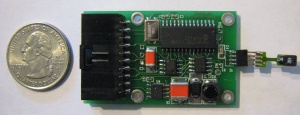
\includegraphics[width =0.5\textwidth]{IcingWarningSensorBoardsm}
\caption{Sensor zur Detektion von Vereisungsbedingungen von Airborne Innovations\cite{AirbInoweb}}
\end{figure}

Angaben zur Vereisungsgefahr in Abh�ngigkeit der Lufttemperatur hat Mindermann in seiner Arbeit festgehalten. Unter -40�C tritt Wasser ausschliesslich in fester Form auf. Die H�lfte aller Vereisungen treten zwischen -12�C und -8�C auf.\cite{Minderthes}
\begin{figure}[H]
\centering
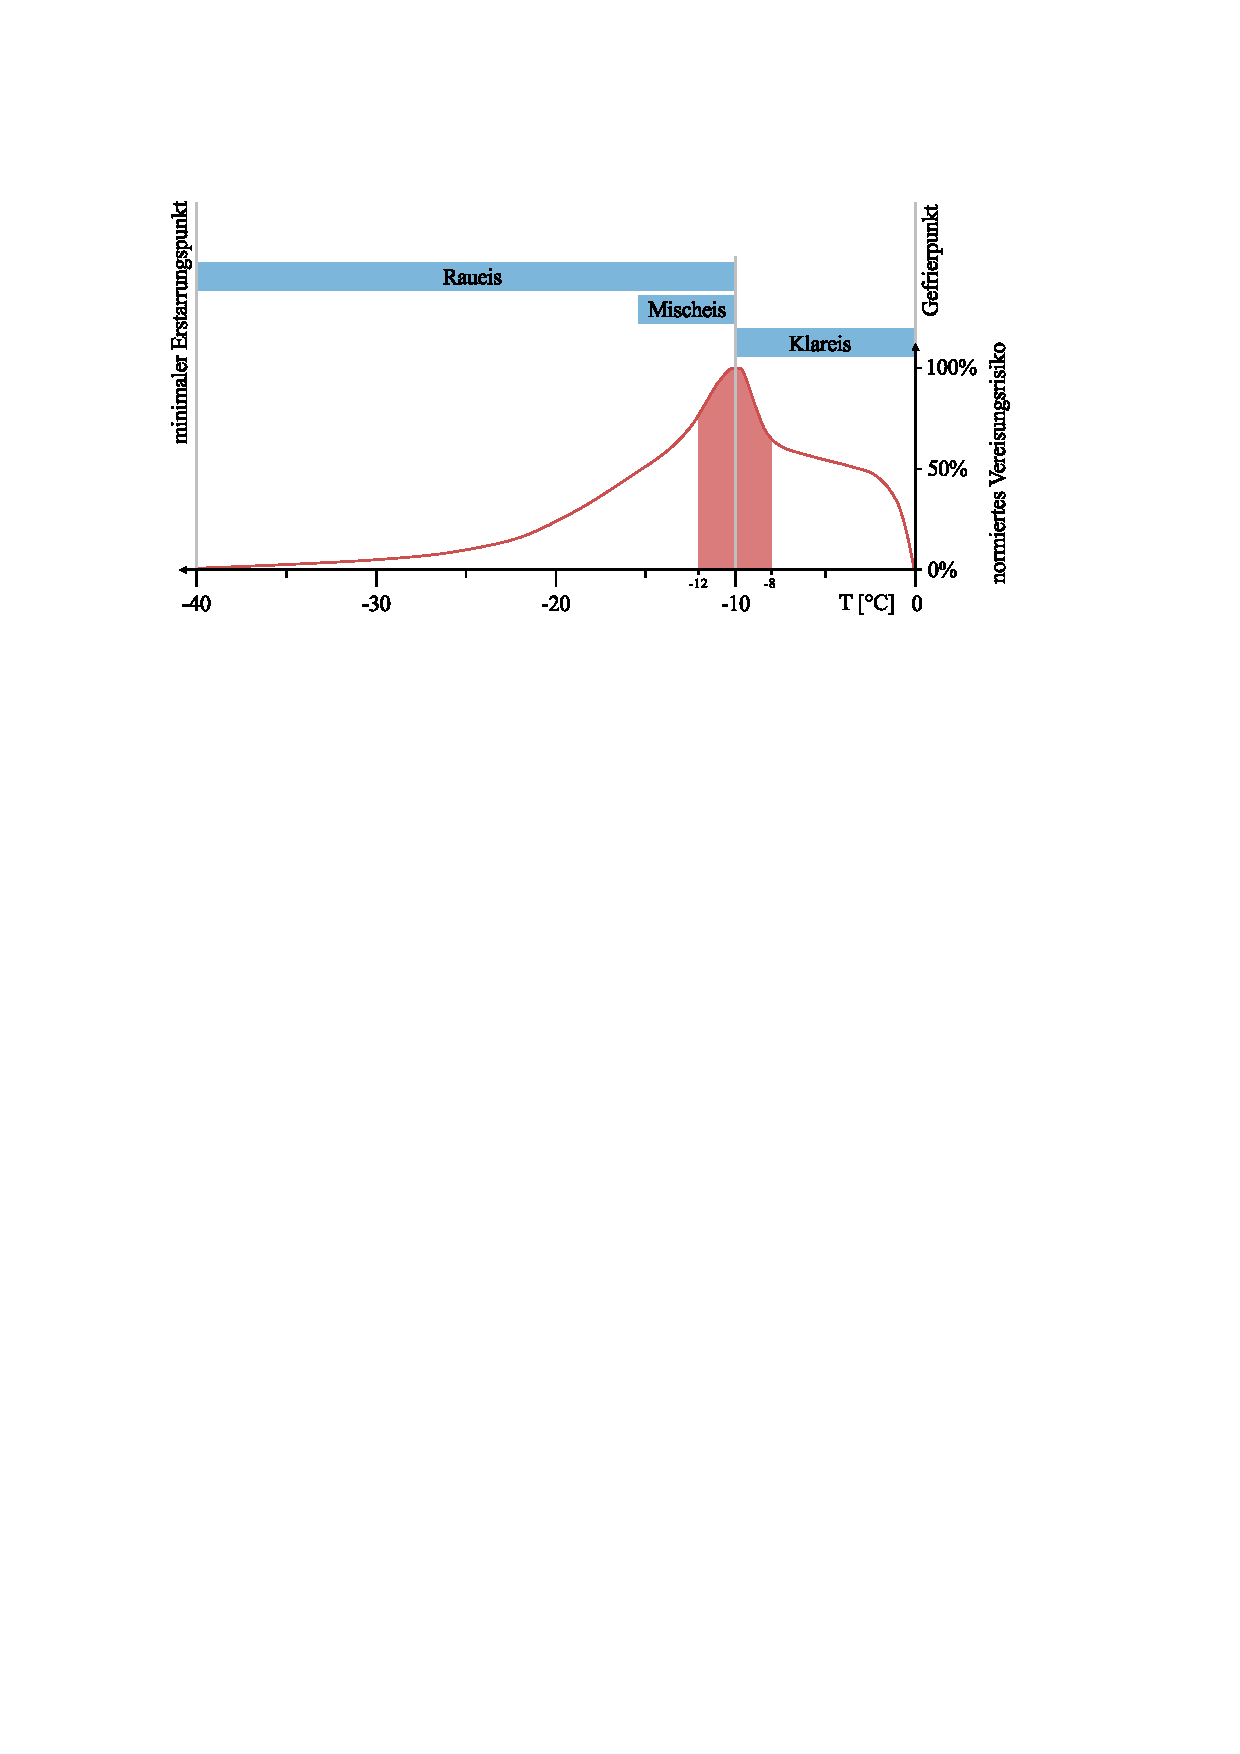
\includegraphics[trim = 0mm 190mm 0mm 30mm,clip,width =1\textwidth]{Vereisungswahrscheinlichkeit}
\caption{Temperaturabh�ngiges auf das Maximum normiertes Risiko einer Flugzeugvereisung
(rot), �bliche Erscheinungsbereiche verschiedener Eisarten
(blau)\cite{Minderthes}}
\end{figure}


\section{Energie�bertragung}
Ein Problem, das vorwiegend bei elektrischer Beheizung des Rotors besteht, ist die Energie�bertragung auf den Rotor. Der Super Puma versorgt �ber einen mehrkontaktigen Schleifring sieben verschiedene Heizsegmente pro Rotor mit Energie\cite{Pumapp}. Der Anspruch an die Schleifkontakte ist aber gross. Der Hauptrotor dreht mit 268\(\frac{1}{min}\)\cite{Swissheliweb} und es wird eine Leistung von 23kW\cite{Pumapp} �bertragen.
Eine alternative M�glichkeit zur �bertragung besteht durch Induktive Drahtlos�bertragung. Eine Spule am Rumpf erzeugt ein Magnetfeld, welches in eine Spule, die am Rotor mit dreht, einen Strom induziert. Solch ein System bedingt hohen Entwicklungsaufwand. Eine mehrkanalige �bertragung ist schwierig zu realisieren. 

\part{Beschrieb der Komponenten}

\section{Aufbau der Komponenten}
\def\svgwidth{0.5\textwidth}
%% Creator: Inkscape inkscape 0.92.3, www.inkscape.org
%% PDF/EPS/PS + LaTeX output extension by Johan Engelen, 2010
%% Accompanies image file 'Komponentendiagramm.eps' (pdf, eps, ps)
%%
%% To include the image in your LaTeX document, write
%%   \input{<filename>.pdf_tex}
%%  instead of
%%   \includegraphics{<filename>.pdf}
%% To scale the image, write
%%   \def\svgwidth{<desired width>}
%%   \input{<filename>.pdf_tex}
%%  instead of
%%   \includegraphics[width=<desired width>]{<filename>.pdf}
%%
%% Images with a different path to the parent latex file can
%% be accessed with the `import' package (which may need to be
%% installed) using
%%   \usepackage{import}
%% in the preamble, and then including the image with
%%   \import{<path to file>}{<filename>.pdf_tex}
%% Alternatively, one can specify
%%   \graphicspath{{<path to file>/}}
%% 
%% For more information, please see info/svg-inkscape on CTAN:
%%   http://tug.ctan.org/tex-archive/info/svg-inkscape
%%
\begingroup%
  \makeatletter%
  \providecommand\color[2][]{%
    \errmessage{(Inkscape) Color is used for the text in Inkscape, but the package 'color.sty' is not loaded}%
    \renewcommand\color[2][]{}%
  }%
  \providecommand\transparent[1]{%
    \errmessage{(Inkscape) Transparency is used (non-zero) for the text in Inkscape, but the package 'transparent.sty' is not loaded}%
    \renewcommand\transparent[1]{}%
  }%
  \providecommand\rotatebox[2]{#2}%
  \newcommand*\fsize{\dimexpr\f@size pt\relax}%
  \newcommand*\lineheight[1]{\fontsize{\fsize}{#1\fsize}\selectfont}%
  \ifx\svgwidth\undefined%
    \setlength{\unitlength}{337.0274005bp}%
    \ifx\svgscale\undefined%
      \relax%
    \else%
      \setlength{\unitlength}{\unitlength * \real{\svgscale}}%
    \fi%
  \else%
    \setlength{\unitlength}{\svgwidth}%
  \fi%
  \global\let\svgwidth\undefined%
  \global\let\svgscale\undefined%
  \makeatother%
  \begin{picture}(1,0.64138133)%
    \lineheight{1}%
    \setlength\tabcolsep{0pt}%
    \put(0,0){\includegraphics[width=\unitlength]{Bilder/Komponentendiagramm}}%
    \put(0.71067542,0.57945568){\color[rgb]{0,0,0}\makebox(0,0)[lt]{\lineheight{1.25}\smash{\begin{tabular}[t]{l}Heizung\end{tabular}}}}%
    \put(0.02357652,0.35460024){\color[rgb]{0,0,0}\makebox(0,0)[lt]{\lineheight{1.25}\smash{\begin{tabular}[t]{l}tiny K22\end{tabular}}}}%
    \put(0.62426972,0.36443615){\color[rgb]{0,0,0}\makebox(0,0)[lt]{\lineheight{1.25}\smash{\begin{tabular}[t]{l}Lufttemperatur\end{tabular}}}}%
    \put(0.61757051,0.14590481){\color[rgb]{0,0,0}\makebox(0,0)[lt]{\lineheight{1.25}\smash{\begin{tabular}[t]{l}Rel. Luftfeuchte\end{tabular}}}}%
    \put(0.1130551,0.03698331){\color[rgb]{0,0,0}\makebox(0,0)[lt]{\lineheight{1.25}\smash{\begin{tabular}[t]{l}SD Karte\end{tabular}}}}%
  \end{picture}%
\endgroup%



\part{Versuche}

\section{Versuch zur Ermittlung der thermischen Energie}
Eine erste Versuchsrunde soll die n�tige Energie zum l�sen von Eis zeigen. Mit einem Heizdraht versehene Proben entsprechen dem Aufbau eines Rotorblatt. Auf gefrorene Stoffst�cke sollen die Eisschicht imitieren. Gewicht das an den Stoffst�cke h�ngt, simuliert die Fliehkraft, die am Rotor auf das Eis wirkt. Die Zeit bis sich der Stoff von der Probe l�st soll zeigen welche Leistung pro Quadratzentimeter sinnvoll ist. Leider geben die Resultate keine sinnvolle Resultate. Die Leistung kann nicht in den Zusammenhang zur Leistung gebracht werden. Auch eine Wiederholung des Versuchs in der Klimakammer bei -10�C Lufttemperatur kann die Resultate nicht verbessern. Die

\section{Versuch zur Eisbildung}
\subsection{Versuchsaufbau}
In der Klimakammer soll durch bespr�hen mit Wasser Eis am drehenden Rotor ansetzen. Bei -10�C und einer relativen Luftfeuchtigkeit im Bereich von rund 80 \% dreht der Rotor mit rund 5000 \(\frac{1}{min}\). Eine D�se zerst�ubt Wasser zu Nebel. Eine Datenlogger zeichnet Die Luftfeucht und die Lufttemperatur nahe dem Rotor auf. Ein Kamera zeichnet das Rotorblatt auf. Zus�tzliche Eindr�cke gibt eine W�rmebildkamera.
\subsection{Resultat}
Auf den Bildern der optischen Kamera l�sst sich lediglich das Einsetzen des Nebels erkennen. Der Rotor dreht zu schnell und ist auf den Bildern verschwommen. Auf den Bildern der W�rmebildkamera ist mangels Kontrast auch nicht zu erkennen. Eine HighSpeed Kamera w�rde die Auswertung zuk�nftiger Versuche beg�nstigen.
Die Eisbildung erfolgt unmittelbar nach dem einschalten des Wasser. Die Stromversorgung des Rotorantrieb l�uft augenblicklich in die Strombegrenzung und die Drehzahl f�llt auf rund 4000\(\frac{1}{min}\).
Das Eis setzt fast ausschliesslich and der Vorderkant in Drehrichtung an. Auf der Vorderseite (in Richtung D�se) ist die Eisschicht bis ca. 12mm von der Kante nach hinten. Auf der Hinterseite (von der D�se abgewandt) ragt die Eisschicht bis 26mm von der Kante weg.

\part{Schlussteil}

\section{Fazit}
Das Ziel der Arbeit, die Funktion einer Enteisungsvorrichtung demonstrieren zu k�nnen, wurde nicht erf�llt. Die Zeit reichte nicht, um nach der Erarbeitung der Grundlagen ein Rotorblatt zu fertigen. Die Organisation von Infrastruktur wie der Klimakammer und die Bereitstellung des Pr�fstands hat die Arbeit verz�gert. Der Prozess zum Herstellen eines Rotorblatts dauert relativ lange, da hierf�r zuerst die spezifischen Werkzeuge f�r die Rotorblattform hergestellt werden m�ssen. Die Resultate bieten trotzdem eine gute Grundlage f�r eine Weiterarbeit. Die n�tige Leistung f�r eine Enteisung durch Beheizen konnte grob abgesch�tzt werden. Es zeigte sich, dass Eis relativ einfach k�nstlich erzeugt werden kann, was kommende Versuche mit einem beheizten Rotorblatt beg�nstigt. Der Prototyp ist bis auf das Heizelement Funktionsf�hig und kann relevante Umgebungsparameter zuverl�ssig aufzeichnen. Er bietet eine solide Grundlage f�r zuk�nftige Tests und ein endg�ltiges Enteisungssystem. 

%% <== Ende der Hinweise
%%%%%%%%%%%%%%%%%%%%%%%%%%%%%%%%%%%%%%%%%%%%%%%%%%%%%%%%%%%%%



%%%%%%%%%%%%%%%%%%%%%%%%%%%%%%%%%%%%%%%%%%%%%%%%%%%%%%%%%%%%%
%% LITERATUR UND ANDERE VERZEICHNISSE
%%%%%%%%%%%%%%%%%%%%%%%%%%%%%%%%%%%%%%%%%%%%%%%%%%%%%%%%%%%%%
%% Ein kleiner Abstand zu den Kapiteln im Inhaltsverzeichnis (toc)
\addtocontents{toc}{\protect\vspace*{\baselineskip}}
\medskip
%% Literaturverzeichnis
%% ==> Eine Datei 'literatur.bib' wird hierf�r ben�tigt.
%% ==> Sie m�ssen hierf�r BibTeX verwenden (Projekt | Eigenschaften... | BibTeX)
\addcontentsline{toc}{section}{Literaturverzeichnis}
\nocite{*} %Auch nicht-zitierte BibTeX-Eintr�ge werden angezeigt.
 %Art der Ausgabe: plain / apalike / amsalpha / ...
\bibliography{Literaturverzeichniss} %Eine Datei 'literatur.bib' wird hierf�r ben�tigt.

%% Abbildungsverzeichnis
\clearpage
\addcontentsline{toc}{section}{Abbildungsverzeichnis}
\listoffigures

%% Tabellenverzeichnis
\clearpage
\addcontentsline{toc}{section}{Tabellenverzeichnis}
\listoftables


%%%%%%%%%%%%%%%%%%%%%%%%%%%%%%%%%%%%%%%%%%%%%%%%%%%%%%%%%%%%%
%% ANH�NGE
%%%%%%%%%%%%%%%%%%%%%%%%%%%%%%%%%%%%%%%%%%%%%%%%%%%%%%%%%%%%%
\appendix
%% ==> Schreiben Sie hier Ihren Text oder f�gen Sie externe Dateien ein.
\part{Anhang}
%\input{Dateiname} %Eine Datei 'Dateiname.tex' wird hierf�r ben�tigt.


\end{document}

